\documentclass{beamer}

\usefonttheme{professionalfonts} % using non standard fonts for beamer
\usefonttheme{serif} % default family is serif

\usepackage{hyperref}

%\usepackage{minted}

\usepackage{animate}

\usepackage{graphicx}

\def\Put(#1,#2)#3{\leavevmode\makebox(0,0){\put(#1,#2){#3}}}

\usepackage{color}

\usepackage{tikz}

\usepackage{amssymb}

\usepackage{enumerate}


\newcommand\blfootnote[1]{%

  \begingroup

  \renewcommand\thefootnote{}\footnote{#1}%

  \addtocounter{footnote}{-1}%

  \endgroup

}

\makeatletter

%%%%%%%%%%%%%%%%%%%%%%%%%%%%%% Textclass specific LaTeX commands.

 % this default might be overridden by plain title style

 \newcommand\makebeamertitle{\frame{\maketitle}}%

 % (ERT) argument for the TOC

 \AtBeginDocument{%

   \let\origtableofcontents=\tableofcontents

   \def\tableofcontents{\@ifnextchar[{\origtableofcontents}{\gobbletableofcontents}}

   \def\gobbletableofcontents#1{\origtableofcontents}

 }

%%%%%%%%%%%%%%%%%%%%%%%%%%%%%% User specified LaTeX commands.

\usetheme{Malmoe}

% or ...

\useoutertheme{infolines}

\addtobeamertemplate{headline}{}{\vskip2pt}



\setbeamercovered{transparent}

% or whatever (possibly just delete it)

\makeatother

\begin{document}
\title[DCEL report]{Parallel DCEL Construction Report}
\author[AC]{Andres Calderon}
\institute[Summer'19]{University of California, Riverside}
\makebeamertitle
\newif\iflattersubsect

\AtBeginSection[] {
    \begin{frame}<beamer>
    \frametitle{Outline} 
    \tableofcontents[currentsection]  
    \end{frame}
    \lattersubsectfalse
}

\AtBeginSubsection[] {
    \begin{frame}<beamer>
    \frametitle{Outline} 
    \tableofcontents[currentsubsection]  
    \end{frame}
}

\begin{frame}{Sweep-line algorithm}
    \begin{itemize}
        \item Using an available implementation from JTS Plus library:
        \begin{itemize}
            \item SimpleMCSweepLineIntersector\footnote{Available at: \url{https://tinyurl.com/y3z37a4c}}: Finds all intersections in one or two sets of edges, using an x-axis sweepline algorithm in conjunction with Monotone Chains. While still $O(n^2)$ in the worst case, this algorithm drastically improves the average-case time. The use of MonotoneChains as the items in the index seems to offer an improvement in performance over a sweep-line alone.
        \end{itemize}

    \end{itemize}
\end{frame}

\begin{frame}{DCEL merger}
    \centering 
    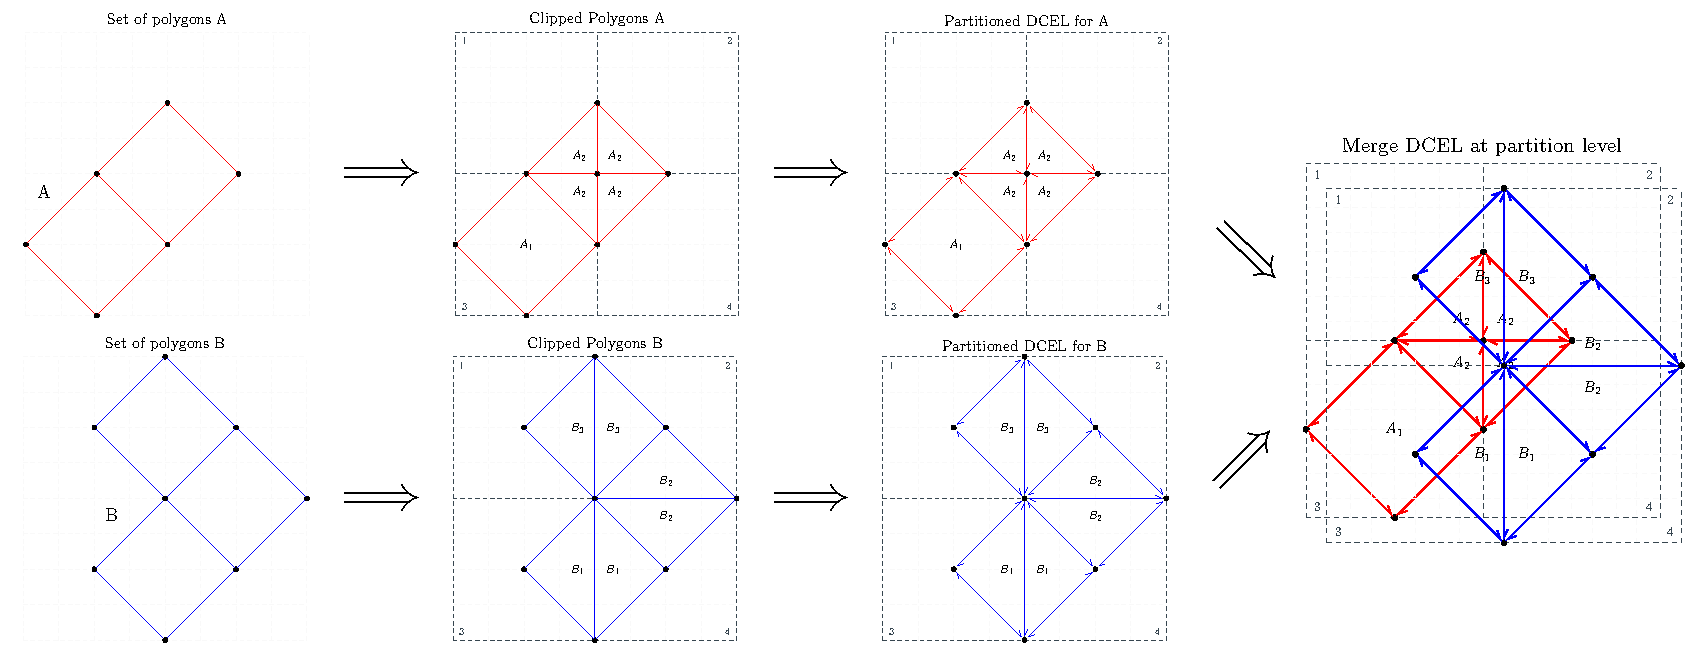
\includegraphics[width=0.9\linewidth]{figures/OverlayParted} 
\end{frame}

\begin{frame}{DCEL merger}
    \centering 
    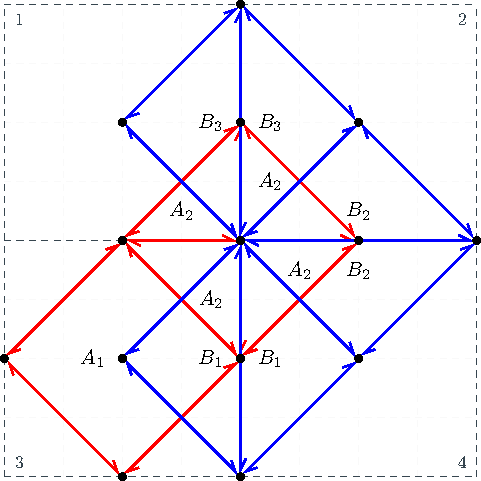
\includegraphics[width=0.5\linewidth]{figures/MergeParts} 
\end{frame}

\begin{frame}{Focus on partition 2}
    \centering 
    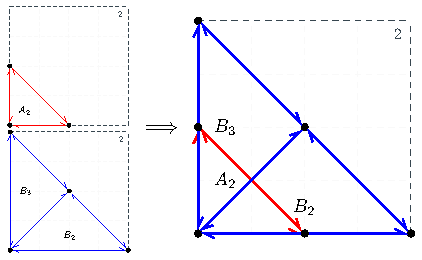
\includegraphics[width=0.9\linewidth]{figures/Part2} 
\end{frame}

\begin{frame}{Focus on partition 2}
    \centering 
    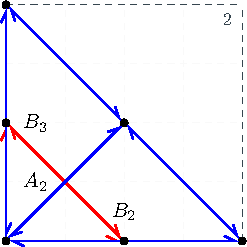
\includegraphics[width=0.6\linewidth]{figures/Part2Overlap} 
\end{frame}

\begin{frame}{Finding intersections}
    \centering 
    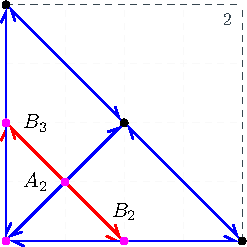
\includegraphics[width=0.6\linewidth]{figures/Part2Intersections} 
\end{frame}

\begin{frame}{Doing splits and grouping duplicates}
    \centering 
    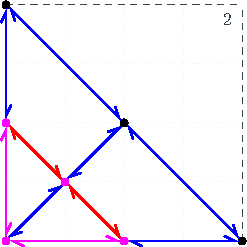
\includegraphics[width=0.6\linewidth]{figures/Part2Splits} 
\end{frame}

\begin{frame}{Collecting vertices and their incidents}
    \centering 
    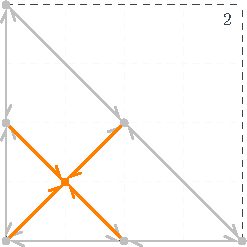
\includegraphics[width=0.6\linewidth]{figures/Part2Incidents} 
\end{frame}

\begin{frame}{What is next}
    \begin{itemize}
        \item Update the pointers (twin, next, prev) for the new vertices (intersections).
        \item Update the face labels.
        \item Finish integration with the current code.
        \item Perform tests.
    \end{itemize}
\end{frame}

\end{document}
